%==============================================================================
\chapter{In silico mapping calcium pharmacological modulations to whole-organ function and model validation}\label{cha:chapter6}
%==============================================================================
%
%
%
\begin{remark}{Outline}
    In this chapter, we investigate how $\Ca$ transient variations can be mapped to the rat whole heart function using the developed emulation framework. We propose to encode the shape of a given $\Ca$ transient using a set of scalar features of clinical interest (Section~\ref{sec:ch6encoding_ca_transient_variations}), allowing these to be quantitatively mapped to the LV features as an additional component to the emulator input parameter set. When using the full forward rat heart contraction model instead, different $\Ca$ transients can be simply plugged-in as new model inputs (previously fixed) to see how they will impact the LV function. Using this second approach, the personalised SHAM rat heart contraction model is validated against known CiPA compounds' effects on $\Ca$ dynamics and how these propagate through to whole heart function (Section~\ref{sec:ch6validating_the_personalised_healthy_rat_heart_model}). We conclude with a brief summary (Section~\ref{sec:ch6summary}).
\end{remark}


%
%
%
\section{Motivation}\label{sec:ch6motivation}
$\Ca$ dynamics plays a key role in the heart contraction and relaxation. We have seen that mapping sarcomere properties to the LV function quantitatively can possibly elucidate the mechanisms that are behind pathological conditions of the heart (Chapter~\ref{cha:chapter4}) and validate pharmacological compounds' mechanisms of action (Chapter~\ref{cha:chapter5}). Building upon this concept, the possibility to quantitatively map also $\Ca$ dynamics alterations to the whole heart behaviour is desirable. In Chapter~\ref{cha:chapter4}, we derived a personalised model of the SHAM rat heart contraction using a fixed $\Ca$ transient as an electrical stimulus. In this Chapter, we aim at incorporating $\Ca$ transient variations in the full simulator map (equation~\ref{eq:fsimul}) in order to understand how different, possibly more pathological $\Ca$ transient phenotypes can impact the LV function.


%
%
%
\section{Encoding $\Ca$ transient variations}\label{sec:ch6encoding_ca_transient_variations}
We used a $4$-feature parametric representation of the $\Ca$ transient that maps to common experimentally measured features. The $4$ features encoded the shape of the $\Ca$ transient, and are summarised in Table~\ref{tab:cafeatures}.

\begin{table}[ht!]
    \myfloatalign
    \begin{tabularx}{\textwidth}{llX}
    \toprule
    \tableheadline{$\Ca$ feature}                  & \tableheadline{Units}                         & \tableheadline{Definition} \\ \midrule
    $\dca$                    & $\SI{}{\micro\Molar}$                   & diastolic $\Ca$ concentration \\
    $\ampl$                   & $\SI{}{\micro\Molar}$                   & $\Ca$ concentration signal amplitude \\
    $\tp$                     & $\SI{}{\milli\second}$                  & time to peak $\Ca$ concentration \\
    $\rtf$                    & $\SI{}{\milli\second}$                  & time to half-maximal relaxation from peak $\Ca$ concentration \\
    \bottomrule
    \end{tabularx}
    \caption{Features encoding the calcium transient shape.}
    \label{tab:cafeatures}
\end{table}

\vspace{0.2cm}\noindent
We wish to sample random sets of these features such that the final samples will uniformly cover the feature space, in order to possibly cover both healthy and pathological $\Ca$ transient phenotypes. For this purpose, we used linear weighs to scale each of the four features from a representative $\Ca$ transient. This parametric encoding of $\Ca$ transient variation ensured that all transients maintained a characteristic $\Ca$ transient morphology.

\vspace{0.2cm}
The specific implementation of this scaling strategy is presented in Algorithm~\ref{alg:cascaling}. Note that \texttt{features} function returns the set of four features given an input $\Ca$ transient; \texttt{concatenate} function returns a $1$D array obtained as the horizontal stack of the given input row $1$D arrays; \texttt{linear\_interpolator} function returns a function whose call method uses $1$D linear interpolation to find the value of new points.

\begin{algorithm}[ht!]
    \caption{Scaling a representative calcium transient (y:=$\Cai(t)$) using linear interpolation.}\label{alg:cascaling}
    \begin{algorithmic} 
    \REQUIRE $t=(t_1,\,\dots,\,t_N),\,y=(y_1,\,\dots,\,y_N),\,\,\textrm{with}\quad t_i,\,y_i\ge 0\,\,\forall\,\,i=1,\dots,\,N$ \\ $p=(p_1,\,\dots,\,p_4),\,\,\textrm{with}\quad p_i\ge 0\,\,\forall\,\,i=1,\dots,\,4$
    \ENSURE $y_{new}\,\,|\,\,(\textrm{features}(t,\,y_{new}))_{i} = p_i\cdot(\textrm{features}(t,\,y))_{i}\quad\forall\,\,i=1,\dots,4$ \\ $\textrm{where}\,\,\textrm{features}(t,\,y) = (\dca,\,\ampl,\,\tp,\,\rtf)$ \\ \vspace{0.2cm}
    \STATE $\dca\,\,\leftarrow\,\,(\textrm{features}(t,\,y))_1$
    \STATE $y_{new}\,\,\leftarrow\,\,p_1\cdot\dca + p_2\cdot(y-\dca)$
    \STATE $i_{max}\,\,\leftarrow\,\,\argmax\limits_{i=1,\dots,\,N}{y}$
    \STATE $T \leftarrow t_{N}$ \\
    \vspace{0.2cm}
    \IF{$\,\, p_3\cdot(t_{i_{max}} - t_{1}) + p_4\cdot(t_{N}-t_{i_{max}})\le T\,\,$}
    \STATE $s\,\,\leftarrow\,\,(p_3 - p_4)\cdot t_{i_{max}}$
    \STATE $t_{tmp}\,\,\leftarrow\,\,\textrm{concatenate}(p_3\cdot (t_{1},\,\dots,\,t_{i_{max}}),\,\,(p_4\cdot t_{i_{max}+1}+s,\,\dots,\,p_4\cdot t_{N-1}+s),\,\,(t_{N}))$
    \STATE $f\,\,\leftarrow\,\,\textrm{linear\_interpolator}(t_{tmp},\, y_{new})$
    \STATE $y_{new}\,\,\leftarrow\,\,f(t)$
    \ELSE
    \PRINT ``Not a valid scaling! Returning original calcium curve."
    \STATE $y_{new}\,\,\leftarrow\,\,y$
    \ENDIF
    \RETURN $y_{new}$
    \end{algorithmic}
\end{algorithm}

\vspace{0.2cm}
Figure~\ref{fig:algintopractice} shows how the algorithm works and how new random calcium transients can be generated.

\begin{figure}[ht!]
    \myfloatalign
    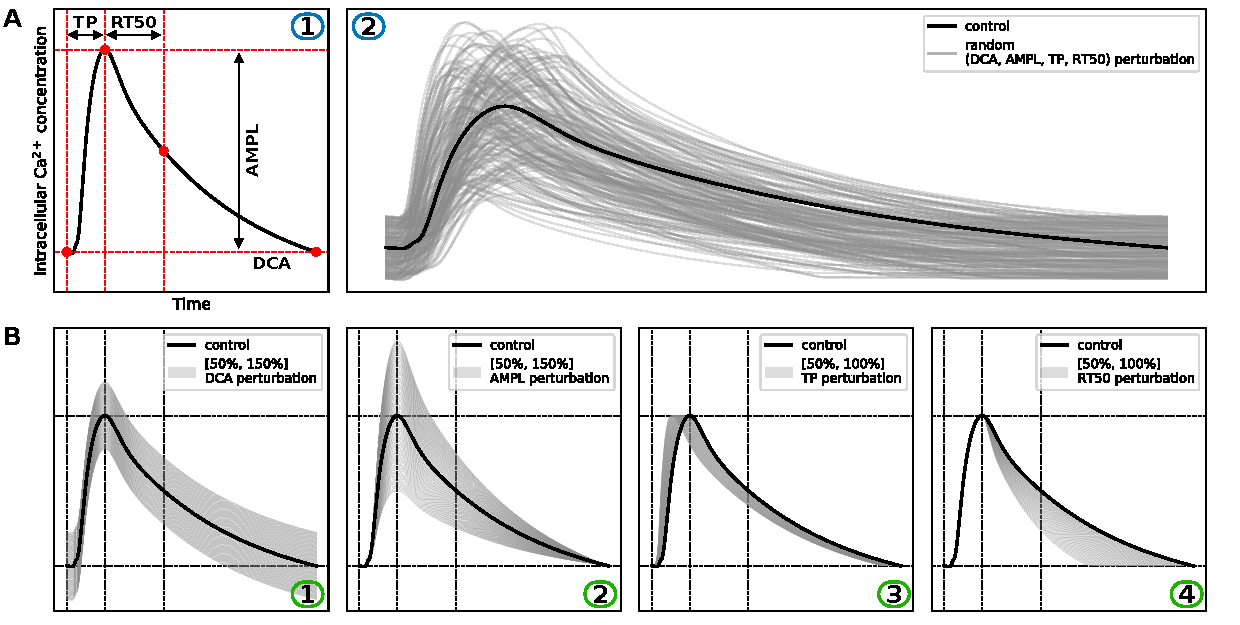
\includegraphics[width=\textwidth]{figures/chapter06/ca_biomarkers_and_scaling_explained_with_labels.pdf}
    \caption{A $4$-feature parametric representation of the calcium transient. (A.1) The calcium transient is described by four relevant quantities: diastolic concentration ($\dca$), amplitude ($\ampl$), time to peak concentration ($\tp$) and time to half-relaxation from peak concentration ($\rtf$). (B.1--4) Each of the $4$ calcium features can be scaled independently to produce a new calcium transient. (A.2) All the features can be scaled at the same time to produce many different new calcium transients.}
    \label{fig:algintopractice}
\end{figure}

\vspace{0.2cm}
An important property of this $\Ca$ scaling strategy is that the features scale linearly with the scaling coefficient used, as shown in Figure~\ref{fig:scalersvscafeatures}. This allows us to randomly sample the scalar parameters that encode the $\Ca$ transient from a space filling design (e.g. a Latin hypercube) while generating samples that cover the full feature space. Having a training dataset with input parameters that uniformly cover the high-dimensional parameter space also helps GP emulators training while at the same time improving their predictions' accuracy.

\begin{figure}[ht!]
    \myfloatalign
    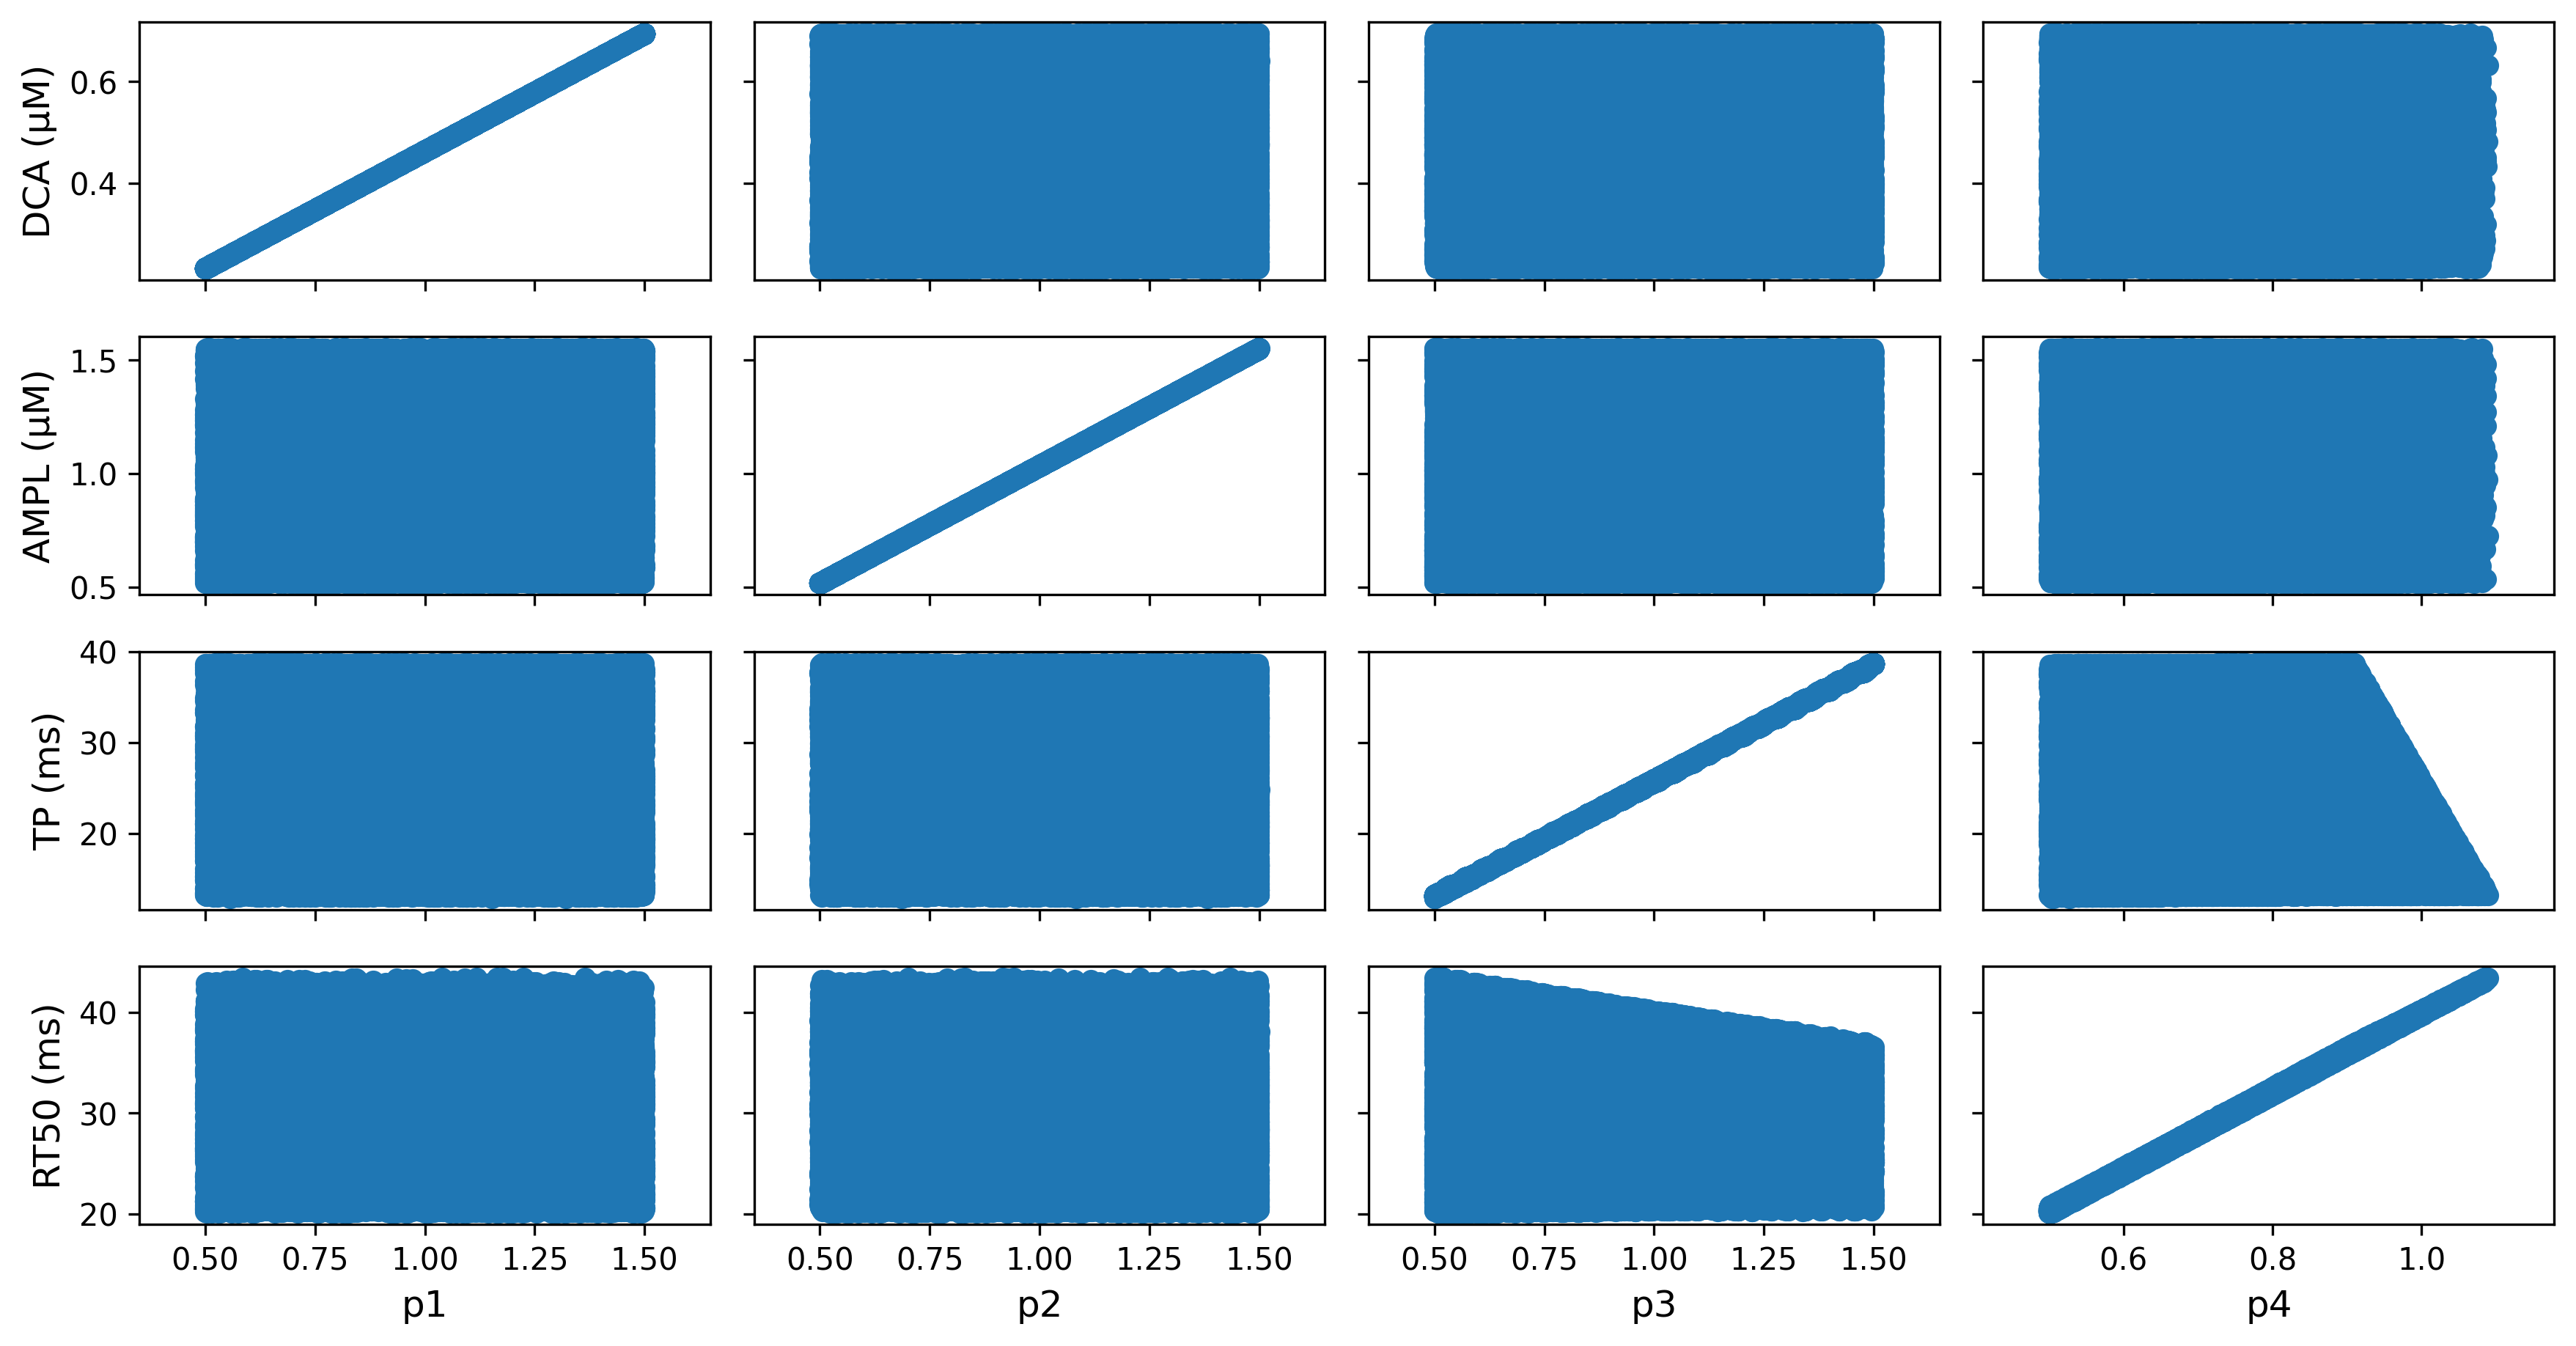
\includegraphics[width=\textwidth]{figures/chapter06/p_vs_b.png}
    \caption{Calcium transient features linearly scale with their respective scaling coefficients. Example showing perturbations in the range $[\SI{50}{\percent},\,\SI{150}{\percent}]$ from control values for all the calcium features but $\rtf$, which undergoes perturbation in the range $[\SI{50}{\percent},\,\SI{110}{\percent}]$.}
    \label{fig:scalersvscafeatures}
\end{figure}

\vspace{0.2cm}
The employed Gattoni et al.~\cite{Gattoni:2017} ionic model simulates a $\Ca$ transient for a fixed pacing rate ($\SI{6}{Hz}$), so that it occurs within a fixed time span. At physiological pacing rates, the rat $\Ca$ transient never reaches an equilibrium in diastole, so that during a $\Ca$ transient time is spent rising or relaxing. As the cell is paced at a fixed cycle length, the sum of time to peak and relaxation time is capped. This means that one cannot increase without the other decreasing, and independent perturbation of $\tp$ and $\rtf$ can only decrease. If relaxation does interdependently slow, this will mean that the cell will not have enough time to fully relax, and this effect is captured by elevating $\dca$ while decreasing $\ampl$. From an algorithmic view point, not all the randomly picked $\Ca$ features' scaling coefficient sets will therefore be viable. The ``if" statement in Algorithm~\ref{alg:cascaling} controls this behaviour by discarding all those curves that decay outside the fixed time interval without fully repolarising.

\vspace{0.2cm}
The existing coupling between $\tp$ and $\rtf$ $\Ca$ features manifests as regions of the feature space that can not be captured by our $\Ca$ transient scaling strategy. These are indicated by the blank triangles in the $p_3$-vs-$\rtf$ and $p_4$-vs-$\tp$ subplots, visible in Figure~\ref{fig:scalersvscafeatures}.


%
%
%
\section{Validating the personalised healthy rat heart model}\label{sec:ch6validating_the_personalised_healthy_rat_heart_model}
To test if the rat heart contraction model can predict how changes in $\Ca$ transients impact the whole heart function, we validated the computational framework by comparing qualitative measurements and predictions of changes in cardiac mechanics in the presence of compounds that manipulate the $\Ca$ transient. This provides a multi-scale test on the ability of the model to map from changes in ion channels conductances to changes in $\Ca$ transient and the resulting changes in whole heart function.

\vspace{0.2cm}\noindent
A schematic of the adopted validation workflow is provided in Figure~\ref{fig:validationschematic}.

\begin{figure}[ht!]
    \myfloatalign
    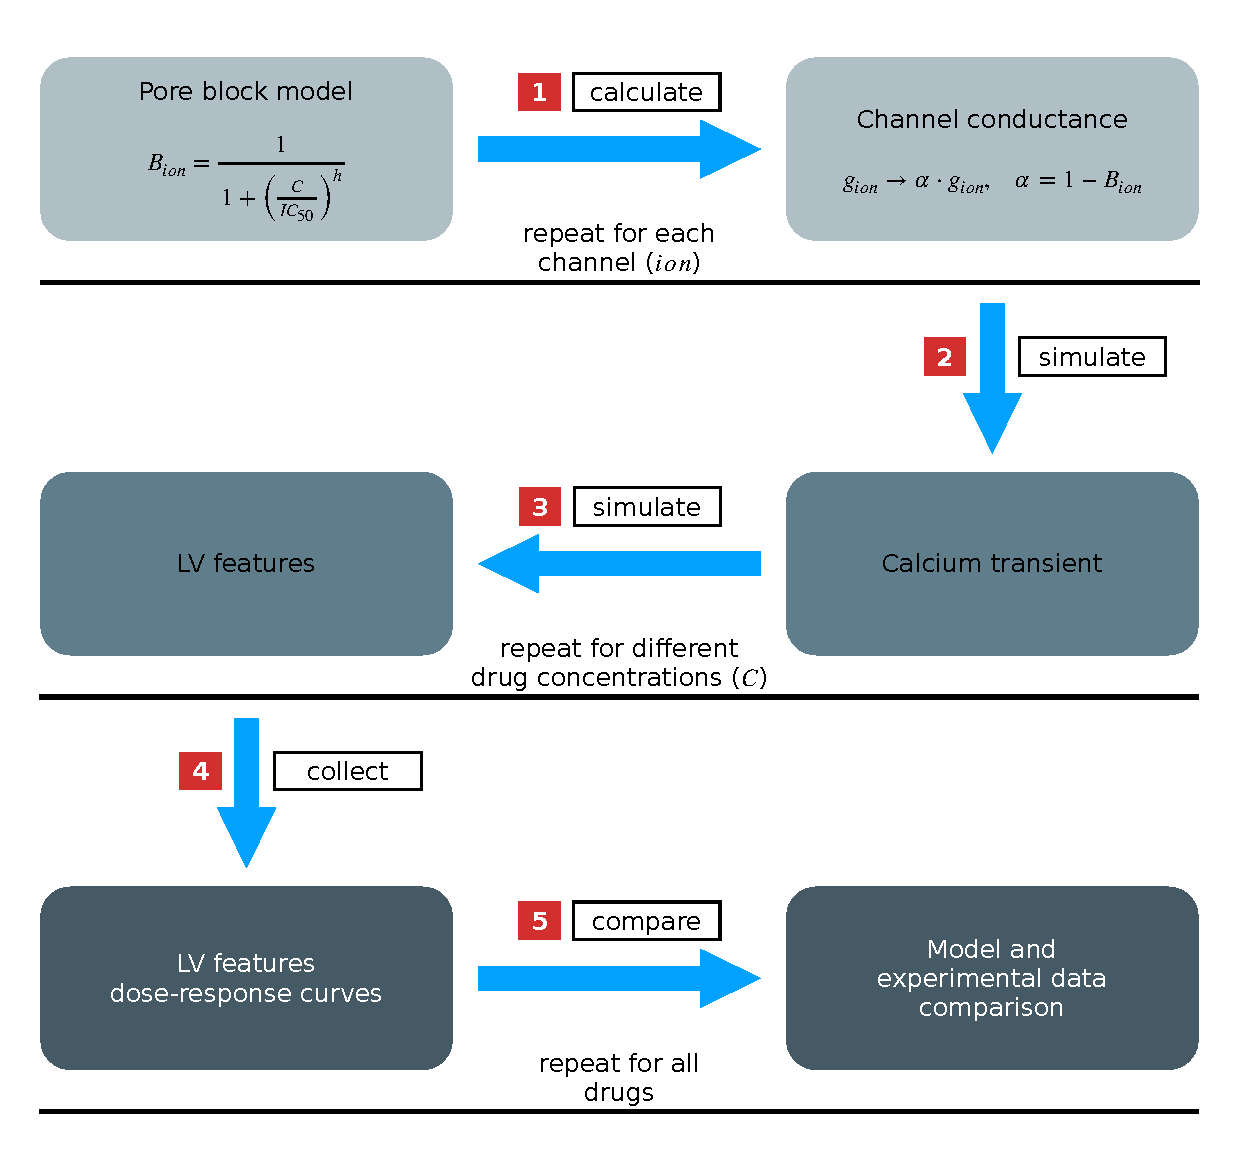
\includegraphics[width=\textwidth]{figures/chapter06/model_validation_schematic.pdf}
    \caption{Model validation workflow. (1) The pore block model is used to calculate the fraction of blocked ion channel at a given compound concentration for each ion channel. The same channels conductances are scaled to reflect this compound effect and (2) the rat myocyte electrophysiological model is run to generate perturbed calcium transients for different compound concentrations. (3) The calcium transients are used as an input for the $3$D biventricular rat heart contraction model and as many LV features' perturbed values are obtained as the number of input curves, which corresponds to the number of tested compound concentrations. (4) Each LV feature values are plotted against the tested compound concentrations to obtain dose-response curves. (5) The qualitative trend of the LV features after \textit{in silico} compound ``administration'' is compared with literature experimentally measured same compound effects on the same LV features for all the compounds under study.}
    \label{fig:validationschematic}
\end{figure}


%
%
%
\subsection{CiPA compounds}\label{sec:ch6cipa_compounds}
We selected $8$ compounds, which were well characterised for multiple ion channels and for which we could find whole organ measurements from literature, from the \textit{comprehensive in vitro proarrhythmia assay} (\acs{CiPA})~\cite{Park:2019} official list, namely bepridil, chlorpromazine, diltiazem, mexiletine, nifedipine, ranolazine, sotalol and verapamil, and we described their action at cellular level using a 4-channel description, namely I\textsubscript{Na}, I\textsubscript{to}, I\textsubscript{K1} and I\textsubscript{CaL}. I\textsubscript{Kr} channel was not included as the related current has a small amplitude in rats cardiomyocytes~\cite{Wymore:1997}, and so was not included in the employed rat cell model~\cite{Gattoni:2017}.

\vspace{0.2cm}
The affinity of each compound for each channel was taken from CiPA project datasets~\cite{Li:2018, Li:2019}, summarised in Table~\ref{tab:compoundporeblock}.

\begin{table}[ht!]
    \myfloatalign
    \begin{tabularx}{\textwidth}{lllll}
    \toprule
    \tableheadline{compound} & \multicolumn{4}{c}{\spacedlowsmallcaps{Ion channel}} \\
    \midrule
    & \tableheadline{I\textsubscript{Na}} & \tableheadline{I\textsubscript{to}} & \tableheadline{I\textsubscript{K1}} & \tableheadline{I\textsubscript{CaL}} \\
    \midrule
    \tableheadline{bepridil}  & & & & \\
    $IC_{50}$ ($\SI{}{\nano\Molar}$)     & $2.93\cdot10^{3}$ & $8.59\cdot10^{3}$ & - & $2.81\cdot10^{3}$ \\
    h                               & $1.16$ & $3.54$ & - & $0.65$ \\ \midrule
    \tableheadline{chlorpromazine}  & & & & \\
    $IC_{50}$ ($\SI{}{\nano\Molar}$)     & $4.54\cdot10^{3}$ & $1.76\cdot10^{7}$ & $9.27\cdot10^{3}$ & $8.19\cdot10^{3}$ \\
    h                               & $2.00$ & $0.37$ & $0.69$ & $0.84$ \\ \midrule
    \tableheadline{diltiazem}       & & & & \\
    $IC_{50}$ ($\SI{}{\nano\Molar}$)     & $1.11\cdot10^{5}$ & $2.82\cdot10^{9}$ & - & $1.12\cdot10^{2}$ \\
    h                               & $0.70$ & $0.17$ & - & $0.71$ \\ \midrule
    \tableheadline{mexiletine}      & & & & \\
    $IC_{50}$ ($\SI{}{\nano\Molar}$)     & - & - & - & $3.82\cdot10^{4}$ \\
    h                               & - & - & - & $1.03$ \\ \midrule
    \tableheadline{nifedipine}      & & & & \\
    $IC_{50}$ ($\SI{}{\nano\Molar}$)     & $2.84\cdot10^{4}$ & - & - & $1.15\cdot10^{1}$ \\
    h                               & $1.11$ & - & - & $0.67$ \\ \midrule
    \tableheadline{ranolazine}      & & & & \\
    $IC_{50}$ ($\SI{}{\nano\Molar}$)     & $6.88\cdot10^{4}$ & - & - & - \\
    h                               & $1.42$ & - & - & - \\ \midrule
    \tableheadline{sotalol}         & & & & \\
    $IC_{50}$ ($\SI{}{\nano\Molar}$)     & $1.14\cdot10^{9}$ & $\SI{4.31e7}{}$ & $3.05\cdot10^{6}$ & $7.06\cdot10^{6}$ \\
    h                               & $0.51$ & $0.66$ & $1.20$ & $0.87$ \\ \midrule
    \tableheadline{verapamil}       & & & & \\
    $IC_{50}$ ($\SI{}{\nano\Molar}$)     & - & $1.34\cdot10^{4}$ & $3.49\cdot10^{8}$ & $2.02\cdot10^{2}$ \\
    h                               & - & $0.82$ & $0.27$ & $1.10$ \\
    \bottomrule                          
    \end{tabularx}
    \caption{$\icf$ and Hill coefficient values describing the affinity of eight CiPA compounds with the I\textsubscript{Na}, I\textsubscript{to}, I\textsubscript{K1} and I\textsubscript{CaL} ion channels. The dash symbol indicates that the specific compound has no inhibitory effect on the respective ion channel. Values taken from~\cite{Li:2018, Li:2019}.}
    \label{tab:compoundporeblock}
\end{table}

\vspace{0.2cm}\noindent
The affinity is described by the Hill coefficient $h$ and the half-maximal inhibitory concentration $\icf$ values of a Hill-type relationship which gives the fraction of blocked current $B$ as a function of the compound concentration $C$, also known as the \textit{pore block model}:
%
\begin{equation}
    B = \frac{1}{1+\left(\frac{C}{\icf}\right)^h}
\end{equation}


%
%
%
\subsection{Compounds' effects on $\Ca$ transient}\label{sec:ch6compounds_effects_on_ca_transient}
For each compound, we calculated $B$ for each channel when $C$ was set to equally-spaced values in a log-molar space. By subtracting the obtained $B$ values from $1$, we obtained a matrix of scaling coefficients for the channels' conductances, representing the fractions of active channels in the presence of the compounds at different concentrations. We tested $13$ equally-spaced values (in $-\log{\SI{}{\Molar}}$ units) in the range $[4,\,10]$ (extremes included), which corresponded to compounds' concentrations between $\SI{e-10}{\Molar}$ and $\SI{e-4}{\Molar}$. We then run the Gattoni et al.~\cite{Gattoni:2017} model by scaling the ion channels' conductances to simulate the action of different concentrations of each compound at cellular level and collected the resulting $\Ca$ transients (last beat curves of limit cycle, $5000$ beats simulations). An example of $\Ca$ transients obtained after simulating the effect of verapamil is provided in Figure~\ref{fig:calciumverapamil}.

\begin{figure}[ht!]
    \myfloatalign
    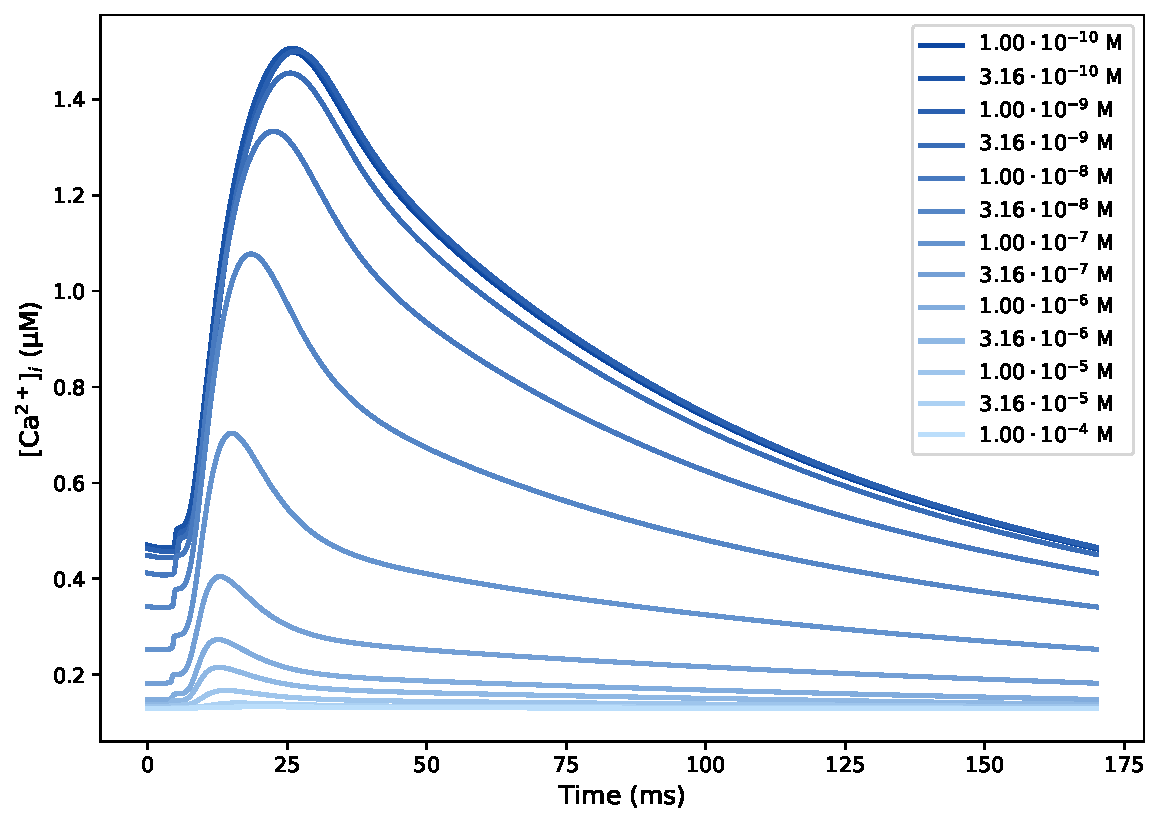
\includegraphics[width=0.8\textwidth]{figures/chapter06/verapamil_calcium_curve_drug.pdf}
    \caption{The effect of verapamil on the intracellular calcium transient. The Gattoni et al.~\cite{Gattoni:2017} model is run using different ion channels' conductances' scaling coefficients to simulate the effect of different concentrations (blue colour variants) of the example compound considered.}
    \label{fig:calciumverapamil}
\end{figure}

\vspace{0.2cm}
As the $\Ca$ transients obtained in the presence of the compound at different concentrations can be encoded by $\dca$, $\ampl$, $\tp$ and $\rtf$ features (Section~\ref{sec:ch6encoding_ca_transient_variations}), we can visualise how these features are varying in a dose-dependent manner. The $\Ca$ transient features' dose-response curves are shown in Figure~\ref{fig:cafeatsverapamilrespcurve} for verapamil.

\begin{figure}[ht!]
    \myfloatalign
    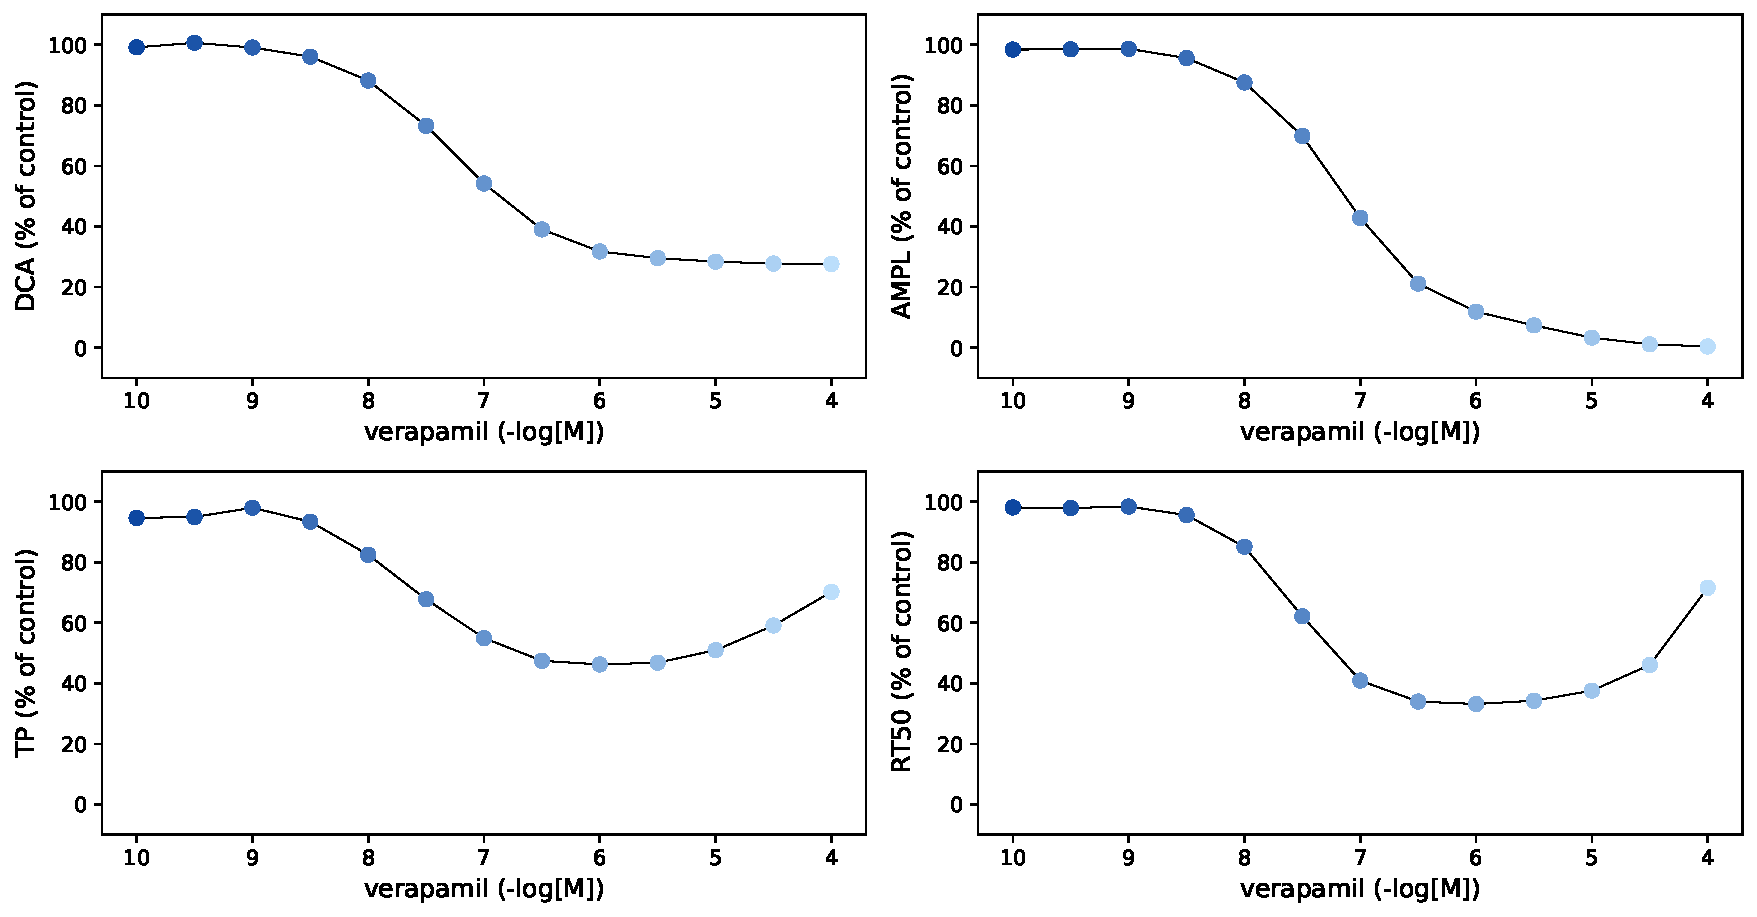
\includegraphics[width=\textwidth]{figures/chapter06/verapamil_dose_calcium_response_curve_drug.pdf}
    \caption{Calcium transient features' dose-response curves. Calcium transient features are extracted from perturbed calcium transients and plotted against the respectively simulated compound concentrations.}
    \label{fig:cafeatsverapamilrespcurve}
\end{figure}

\vspace{0.2cm}\noindent
We can notice that for the $\tp$ and $\rtf$ features the response is not following a fully logistic trend on the right branches. This is because for high compound concentrations we have seen (Figure~\ref{fig:calciumverapamil}) that the $\Ca$ signal had almost vanished, making the analysis of these curves challenging.


%
%
%
\subsection{Compounds' effects on whole-organ function}\label{sec:ch6compounds_effects_on_the_whole_organ_function}
We finally used the personalised healthy (SHAM) rat model (Section~\ref{sec:ch4fittedmodels}) to simulate the LV features' values using as an input the obtained $\Ca$ transients and the remaining parameters fixed to the reference values (Table~\ref{tab:shamabbestfitparamvalues}). This allowed us to obtain the LV features' change from baseline values in a dose-dependent manner. PeakP, maxdP and mindP features' simulated responses to different doses of all the tested compounds are reported in Figure~\ref{fig:LVRVfeatsalldrugsrespcurves}. We additionally extracted the same features' values from the RV limit cycle solution to see if the compound-induced variations were consistent with what observed for the LV. These are provided in the same figure. Moreover, the simulated LV features' percentage changes were compared with quantitative experimental measurements~\cite{Amsterdam:1988,Langslet:1971,Koltai:1989,Saponara:2007,Wang:2007,Kolar:1990} of compounds' effects when these were available from literature (Section~\ref{sec:ch6model_simulated_compounds'_effects_on_whole-organ_function_comparison_with_experimental_observations}, Table~\ref{tab:compoundvalidationrefs}). In particular, in the same figure we report experimental observations for bepridil and verapamil -- PeakP~\cite{Amsterdam:1988}, chlorpromazine -- PeakP~\cite{Langslet:1971}, diltiazem -- PeakP and maxdP~\cite{Koltai:1989}, nifedipine -- PeakP~\cite{Saponara:2007}, ranolazine -- PeakP, maxdP and mindP~\cite{Wang:2007}, and verapamil -- maxdP~\cite{Kolar:1990}.

\begin{figure}[ht!]
    \myfloatalign
    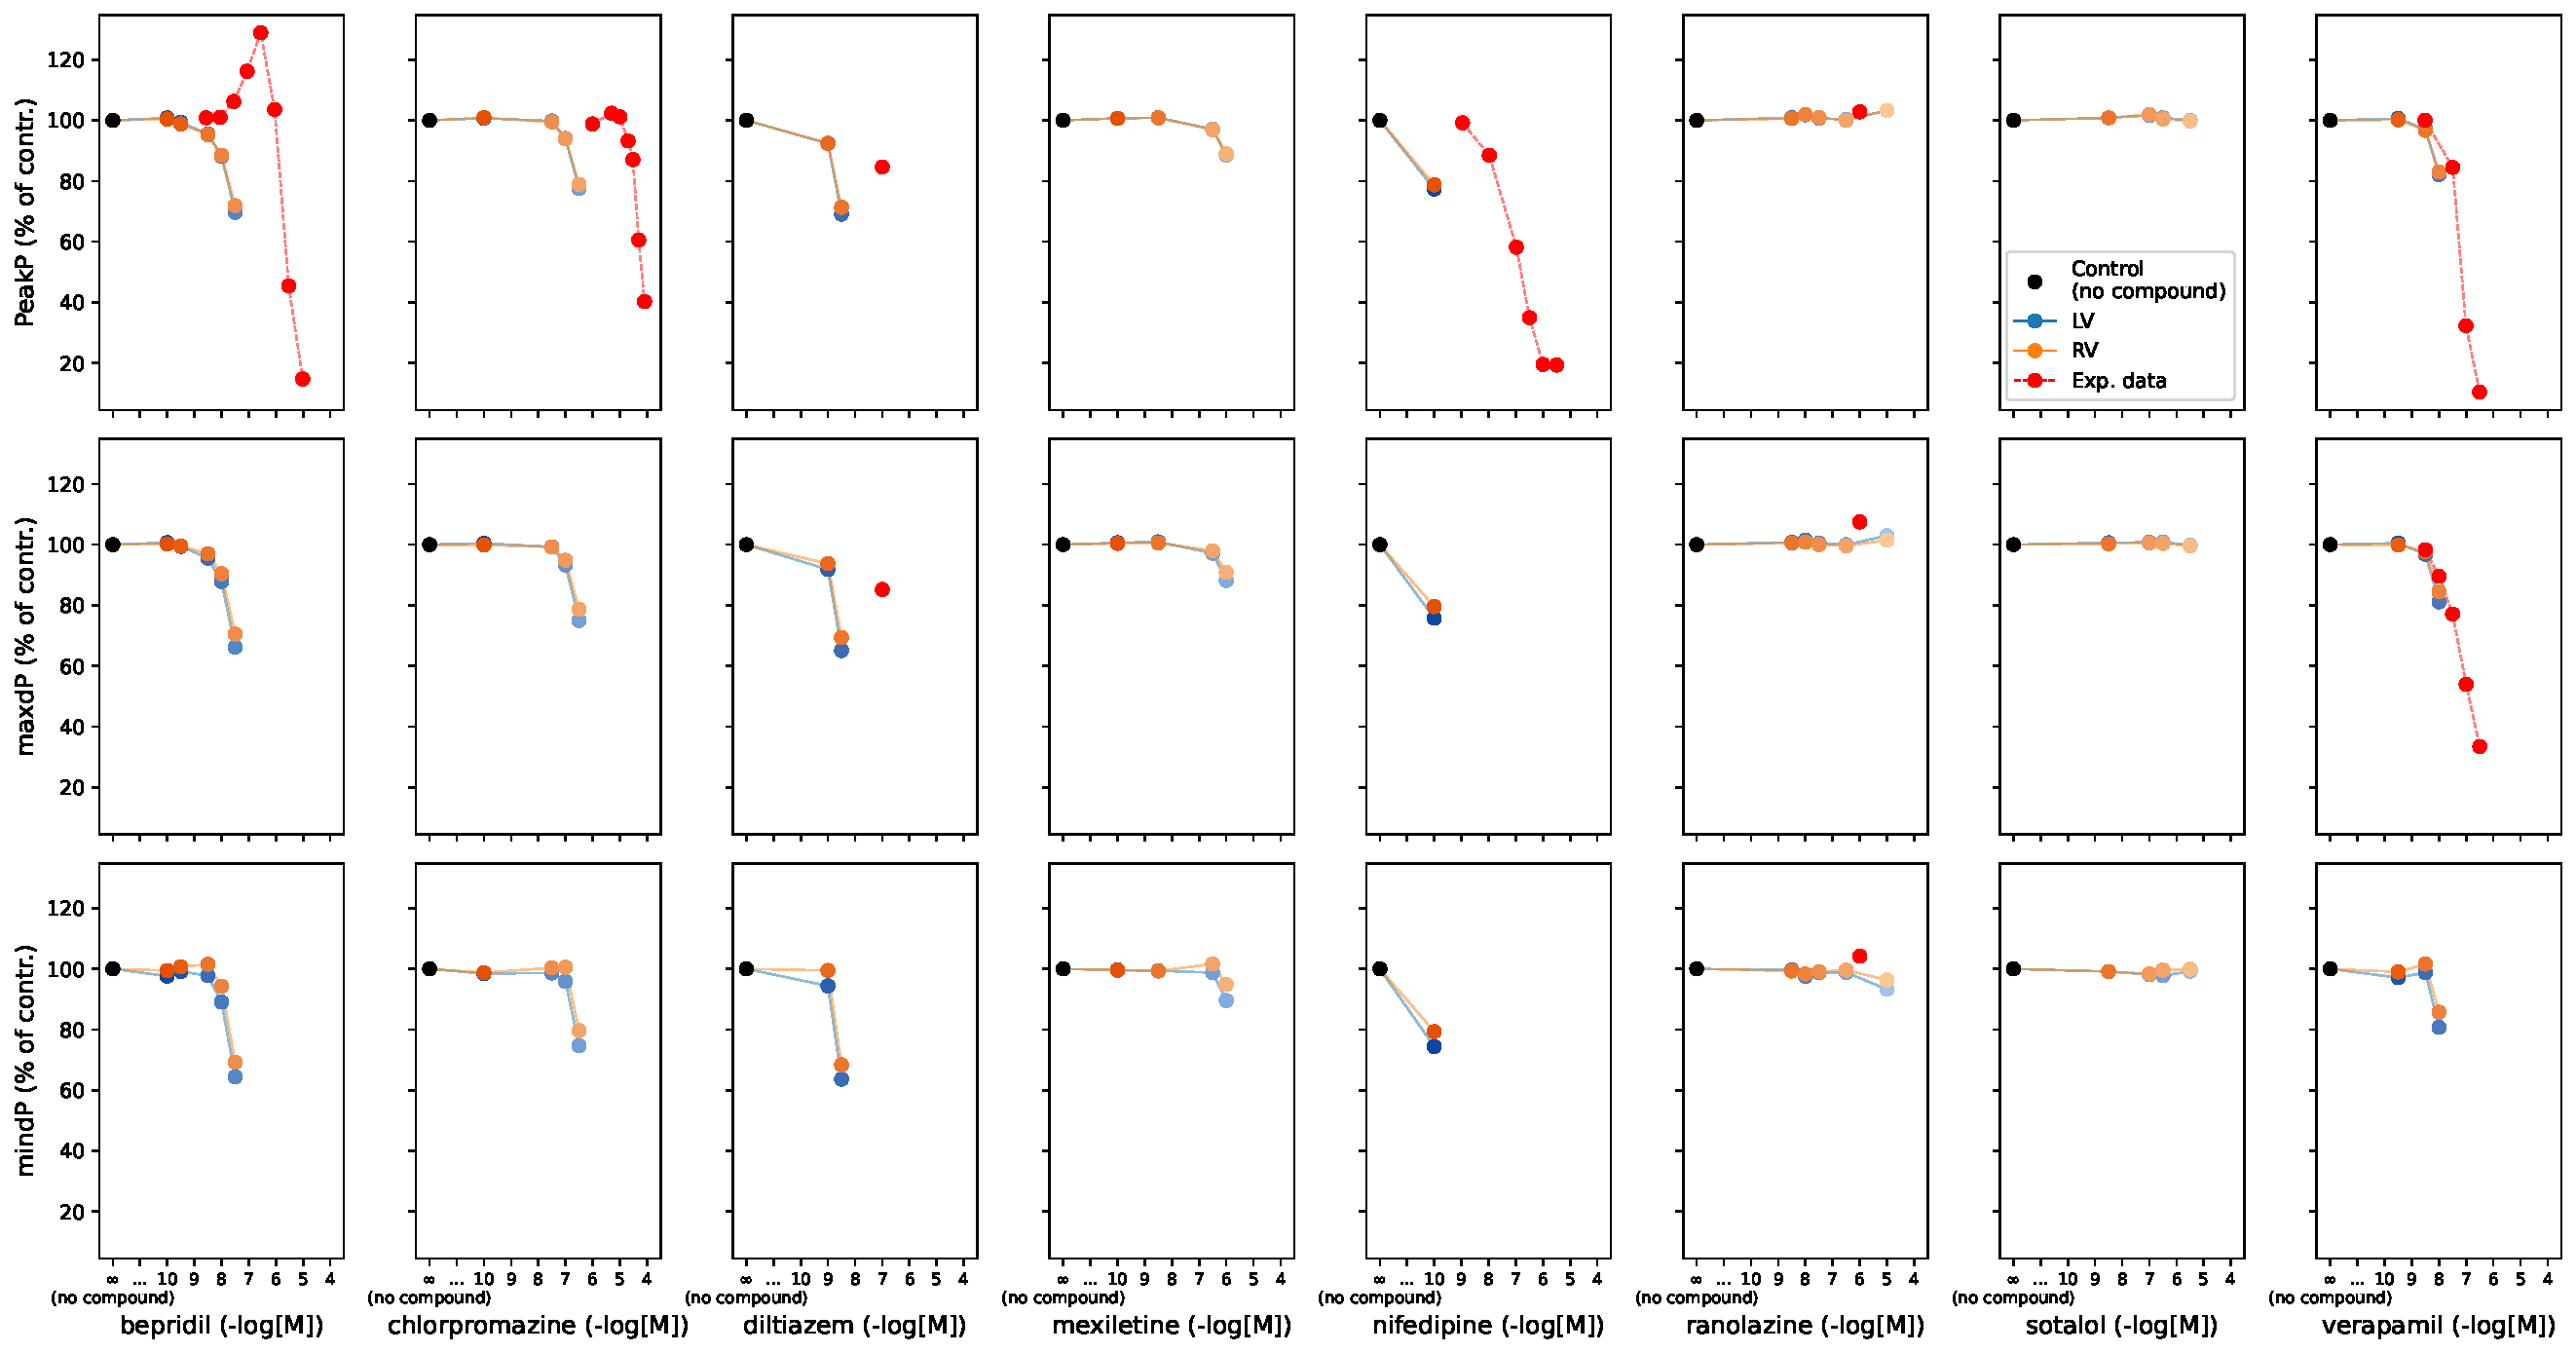
\includegraphics[width=\textwidth]{figures/chapter06/simulated_cipa_compounds_effects_on_lv_rv_pressure_features_with_expdata.pdf}
    \caption{LV and RV pressure features' dose-response curves for the eight CiPA compounds. Simulated PeakP, maxdP and mindP features' values are given as percentages of the respective control values, and are represented as dots in blue/orange variants, colour-coded with the compound doses for respectively the left/right ventricles. Black dots indicate the control values when no compound is present. Experimental data of compounds' effects on the LV (when available) is also displayed as red dots.}
    \label{fig:LVRVfeatsalldrugsrespcurves}
\end{figure}

\vspace{0.2cm}
The \textit{in silico} obtained compounds' effects on the considered pressure features were consistent in both the LV and RV, and showed either a decreasing or unchanged trend from baseline values with increasing compounds' concentrations. Experimental data (highlighted in red in Figure~\ref{fig:LVRVfeatsalldrugsrespcurves}) confirmed the trend simulated by the simulator, although with a non-negligible mismatch in the absolute values (see~Section\ref{sec:ch6discussion} for discussion) for bepridil, chlorpromazine, diltiazem and nifedipine compounds (more pronounced) and ranolazine and verapamil compounds (mild).


%
%
%
\subsection{Simulated compounds' effects on LV function comparison with experimental observations}\label{sec:ch6model_simulated_compounds'_effects_on_whole-organ_function_comparison_with_experimental_observations}
The LV pressure features' qualitative responses after \textit{in silico} compound ``administration'' were compared to qualitative changes in the same LV features observed after compounds administration in literature experimental studies performed on either conscious, or Langendorff-perfused or working healthy rat heart preparations. These experimental changes were either recorded after a single dose in the pre-ischaemic phase of an ischaemia-reperfusion experiment, or in a dose-dependent manner, and are summarised in Table~\ref{tab:compoundvalidationrefs}.

\begin{table}[ht!]
    \myfloatalign
    \begin{tabularx}{\textwidth}{lcccl}
    \toprule
    \tableheadline{compound}           & \multicolumn{3}{c}{\spacedlowsmallcaps{LV feature}} & \tableheadline{References} \\
    \midrule
    & PeakP & maxdP & mindP & \\
    \midrule
    bepridil       & $\downarrow$ & $-$ & $-$ & \cite{Leiris:1984, Amsterdam:1988, Huizer:1987} \\
    chlorpromazine & $\downarrow$ & $-$ & $-$ & \cite{Katsuoka:1989, Langslet:1971, Sakai:2017} \\
    diltiazem      & $\downarrow$ & $\downarrow$ & $\downarrow$ & \cite{Flaim:1982, Koltai:1989, Dong:1997} \\
    mexiletine     & $\leftrightarrow$ & $\downarrow$ & $-$ & \cite{Kamiyama:1995, Hesketh:2020, Marshall:1981} \\
    nifedipine     & $\downarrow$ & $\downarrow$ & $\downarrow$ & \cite{Dong:1997, Saponara:2007, Nishimura:1992} \\
    ranolazine     & $\leftrightarrow$ & $\leftrightarrow$ & $\leftrightarrow$ & \cite{Wang:2007, Hwang:2009, Wang:2019} \\
    sotalol        & $\downarrow$ & $\downarrow$ & $\leftrightarrow$ & \cite{Mackin:2019, Hoffmeister:1988, Lamontagne:1989} \\
    verapamil      & $\downarrow$ & $\downarrow$ & $\downarrow$ & \cite{Simonovic:2019, Stojic:2017, Kolar:1990} \\
    \bottomrule
    \end{tabularx}
    \caption{Qualitative change in three LV pressure features observed in literature rat experiments for eight different CiPA compounds. Down-facing arrow means that the specific LV feature decreases from its control value with the specific compound; left-right arrow means that the compound has no effect on that feature; dash symbol means that the specific information could not be retrieved from literature.}
    \label{tab:compoundvalidationrefs}
\end{table}

\vspace{0.2cm}
The comparison of qualitative model predictions to experimental observations is shown in Figure~\ref{fig:validationtable}. The model correctly predicted $16$ out of $19$ ($\SI{84}{\percent}$) experimental observations, with $5$ observations missing data, matching $6$ out of $8$ compounds. Model predictions were never opposite to observations, with either the model or observations reporting no-change when the model failed.

\begin{figure}[ht!]
    \myfloatalign
    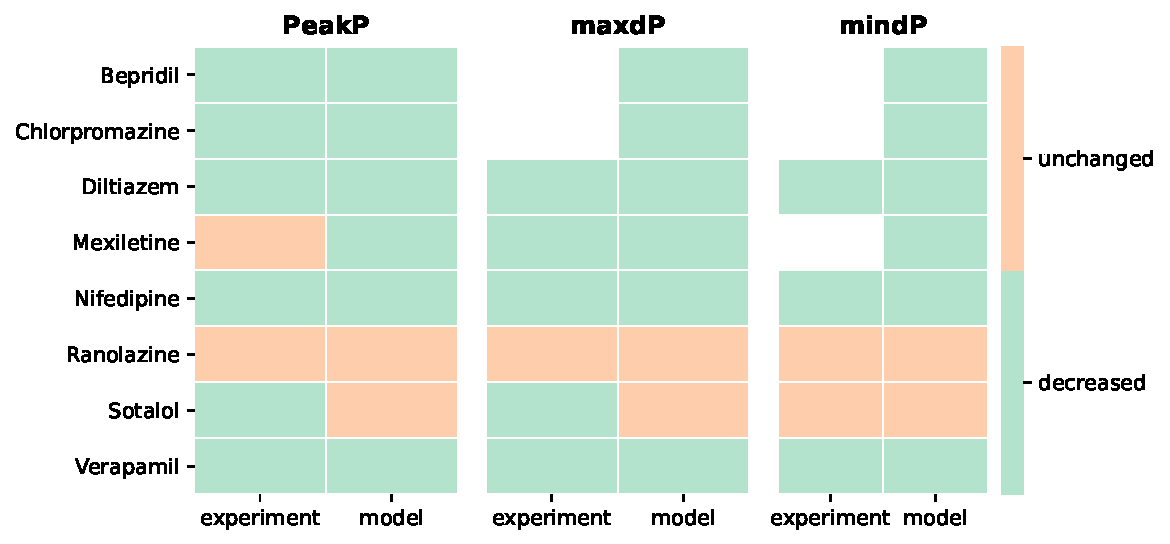
\includegraphics[width=\textwidth]{figures/chapter06/model_vs_experiments.pdf}
    \caption{Model validation against known CiPA compounds effects on whole-organ function. Eight CiPA compounds effects (``experiment" columns) on PeakP, maxdP and mindP are compared with model same compounds' predicted effects on the same features (``model" columns). compounds' effects are colour-coded as orange (feature unchanged) and green (feature decreased). None of the compounds caused an increase in the considered LV features. White/empty space means that the specific effect could not be retrieved from the examined literature studies. Model predicted effects are in agreement with the experimentally observed effects for $6$ out of $8$ compounds.}
    \label{fig:validationtable}
\end{figure}


%
%
%
\section{Discussion}\label{sec:ch6discussion}
The used approach simulates the compound induced changes in the $\Ca$ transient, thereby overcoming the issue when no directly recorded $\Ca$ transients are available. In so doing, we created a fully simulated map from compound properties to whole organ function. \todo{write about mismatch}


%
%
%
\subsection{Limitations}\label{sec:ch6limitations}
Most of the compounds we tested were calcium channel blockers, which are known to reduce the heart rate. Although this can be neutralised by secondary effects such as a reflex increase in beta adrenergic tone in response to systemic vascular dilation, so that because of the level of reflex beta adrenergic discharge the net effect on heart rate could be balanced out~\cite{Low:1982}, our model doesn't account for heart rate variations, so the validation was performed by evaluating the effects of compounds at a fixed, physiological rate. The negative chronotropic effect, coupled with the impact calcium channel blockers have on muscle sympathetic nerve activity~\cite{Binggeli:2002}, can also partially explain the mismatch observed (Figure~\ref{fig:LVRVfeatsalldrugsrespcurves}) when quantitatively comparing compounds' effects onto LV pressure features with the model simulations. Another source of mismatch can be linked to the fixed LV volume setup normally used in the considered experimental studies to evaluate the compounds' effects, which differ from our rat heart model.


%
%
%
\section{Summary}\label{sec:ch6summary}
Having a validated, personalised model of rat heart contraction is powerful as it can be trusted when this is used to predict compounds' mechanisms of action or for identifying in silico pharmacological cellular targets, as we shall see in the next chapter.